\index{Add!Test Cases}
\index{Test Case!Add}
\index{Add!Test Suite}
\index{Test Suite!Add}

You can add (reference) \gdcases{} in other \gdcases{} and in \gdsuites{}. You can also add (reference) \gdsuites{} in \gdjobs{}. 

To add items to an editor:

\begin{enumerate}
\item Open the editor by double-clicking the item you want to add things to.
\item You can now:
\begin{enumerate}
\item Add items via drag and drop from the browser into the editor:

\textbf{\gdcases}:\\
\gdcases{} can be added to other \gdcases{} and \gdsuites{} by selecting the \gdcase{} from the \gdtestcasebrowser{} and dragging it into the editor. 

\textbf{\gdsuites}:\\
\gdsuites{} can be referenced in \gdjobs{} by selecting the \gdsuite{} to reference from the \gdtestsuitebrowser{} and dragging it into the \gdjobeditor{}.

\bxtipp{Once you have added a \gdsuite{} to a \gdjob{}, you must enter the \gdaut{} ID for the \gdaut{} to be tested in the \gdpropview{}.}


\item For \gdcases{}, you can also use the \bxname{Reference Existing \gdcase{}} dialog. Using the context-sensitive menu in the editor, select:\\

\bxmenu{Reference Existing \gdcase{}}{}{}\\

\bxtipp{You can also press \bxkey{ENTER} in the editor to open the \bxname{Reference Existing \gdcase{} dialog.}}

Using this dialog \bxfigref{referencetestcasedialog}, you can choose a \gdcase{} or \gdcases{} to add to the editor. You can filter in through the dialog using the field at the top. Use star \bxshell{*} as a wild card.

\begin{figure}[h]
\begin{center}
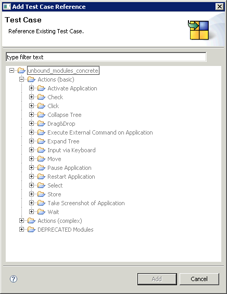
\includegraphics{Tasks/Editors/PS/referencetestcasedialog}
\caption{Add \gdcase{} reference dialog}
\label{referencetestcasedialog}
\end{center}
\end{figure} 

\end{enumerate}
\end{enumerate}

Items you reference in editors are marked with a small arrow to show that they are reused (referenced) here. The name of the item is contained in angled brackets (\bxshell{< >}) to show that it is the same name that you used when you specified the \gdcase{}. Items can be renamed to reflect their particular use in this editor \bxpref{TasksEditorRename}.

\bxwarn{You can't add items which would cause an infinite loop.}
